\section{The preceptron}

\subsection*{Problem 5}
\[
w_{k+1}=\begin{cases}
w_{k}+x_{k} & if\, t_{k}=+1\\
w_{k}-x_{k} & if\, t_{k}=-1
\end{cases}
\]
\[
b_{k+1}=\begin{cases}
b_{k}+1_{k} & if\, t_{k}=+1\\
b_{k}-1_{k} & if\, t_{k}=-1
\end{cases}
\]


\subsection*{Problem 7}
\[
\tilde{w}^{T}w_{k}=\tilde{w}^{T}\left(w_{k-1}+t_{k-1}x_{k-1}\right)=\tilde{w}^{T}\left(w_{k-2}+t_{k-2}x_{k-2}+t_{k-1}x_{k-1}\right)
\]
\[
\tilde{w}^{T}w_{k}=\tilde{w}^{T}\sum_{i=0}^{k-1}t_{i}x_{i}
\]
\[
\tilde{w}^{T}w_{k}=\sum_{i=0}^{k-1}t_{i}\tilde{w}^{T}x_{i}
\]
by knowing that $t_{i}\tilde{w}^{T}x_{i}\geq \gamma$ we can assert
the following
\[
\tilde{w}^{T}w_{k}=\sum_{i=0}^{k-1}t_{i}\tilde{w}^{T}x_{i} \geq \sum_{i=0}^{k-1}\gamma = k\gamma
\]


\subsection*{Problem 8}
\[
\left\Vert w_{k}\right\Vert ^{2}<kR^{2}
\]
from problem 7 we know that $w_{k}=\sum_{i=0}^{k-1}t_{i}x_{i}$ hence
we can write 
\[
\left\Vert \sum_{i=0}^{k-1}t_{i}x_{i}\right\Vert ^{2} \leq kR^{2}
\]
by using the triangle inequality
$\left|A+B\right|\leq\left|A\right|+\left|B\right|$
we can be sure that $\left\Vert \sum_{i=0}^{k-1}t_{i}x_{i}\right\Vert ^{2}$
is smaller or equal than $kR^{2}$.



\subsection*{Problem 9}
We can rewrite $\tilde{w}^{T}w_{k}$ by using problem 7 as 
\[
\left\Vert \tilde{w^{T}}\right\Vert \left\Vert w_{k}\right\Vert
cos(\alpha)=\left\Vert \tilde{w^{T}}\right\Vert \left\Vert
\sum_{i=0}^{k-1}t_{i}x_{i}\right\Vert cos(\alpha)
\]
from problem 7 we know that $\tilde{w}^{T}w_{k}\geq k\gamma$ then
\[
k\gamma\leq\left\Vert \tilde{w^{T}}\right\Vert \left\Vert
\sum_{i=0}^{k-1}t_{i}x_{i}\right\Vert cos(\alpha)
\]
from problem 8 we have $\left\Vert w_{k}\right\Vert ^{2}<kR^{2}$,
thus 
\[
k\gamma\leq\left\Vert \tilde{w^{T}}\right\Vert \left\Vert
\sum_{i=0}^{k-1}t_{i}x_{i}\right\Vert cos(\alpha)
\]
\[
\left(k\gamma\right)^{2}\leq\left(\left\Vert \tilde{w^{T}}\right\Vert
\left\Vert \sum_{i=0}^{k-1}t_{i}x_{i}\right\Vert
cos(\alpha)\right)^{2}<\left\Vert \tilde{w^{T}}\right\Vert
^{2}kR^{2}cos^{2}(\alpha)
\]
\[
k\leq\frac{\left\Vert \tilde{w^{T}}\right\Vert
^{2}R^{2}cos^{2}(\alpha)}{\gamma^{2}}\leq\frac{\left\Vert
\tilde{w^{T}}\right\Vert ^{2}R^{2}}{\gamma^{2}}
\]
  
\newpage
\subsection*{Problem 10}
The data are not separable with the perceptron algorithm because the convex
hulls formed by the points intersect and as it was shown in problem 1 if this 
happens the data are not lineraly separable.
\begin{figure}
\centering{}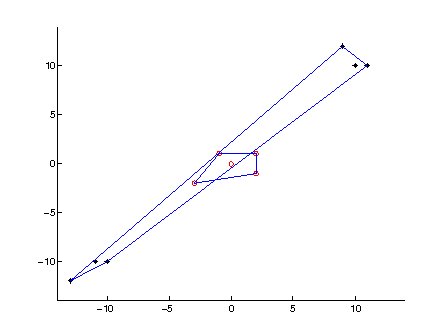
\includegraphics[width=1\textwidth]{plots/10_hull}\caption{Hulls}
\end{figure}

\newpage
\subsection*{Problem 6}
\begin{figure}
\centering{}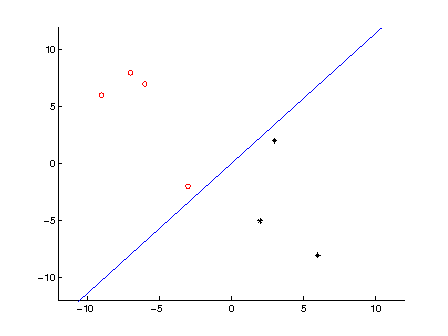
\includegraphics[width=1\textwidth]{plots/6_1}\caption{Problem 6 step 1}
\end{figure}
\begin{figure}
\centering{}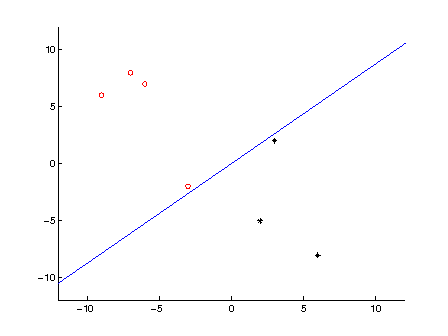
\includegraphics[width=1\textwidth]{plots/6_2}\caption{Problem 6 step 2}
\end{figure}
\begin{figure}
\centering{}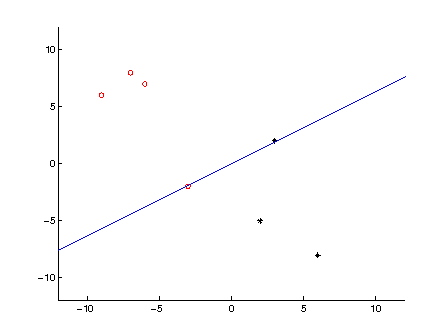
\includegraphics[width=1\textwidth]{plots/6_3}\caption{Problem 6 step 3}
\end{figure}
\begin{figure}
\centering{}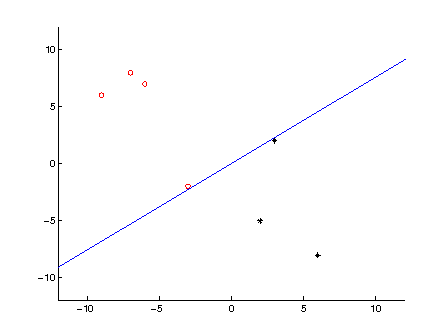
\includegraphics[width=1\textwidth]{plots/6_4}\caption{Problem 6 step 4}
\end{figure}
\begin{figure}
\centering{}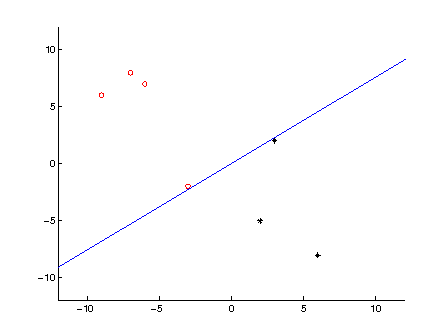
\includegraphics[width=1\textwidth]{plots/6_4}\caption{Problem 6 step 5}
\end{figure}
\begin{figure}
\centering{}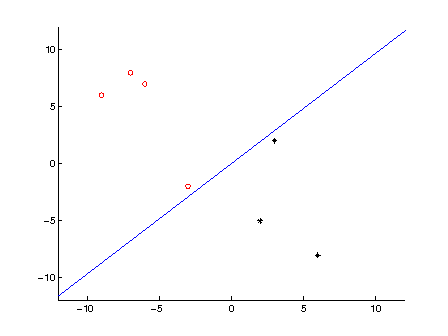
\includegraphics[width=1\textwidth]{plots/6_6}\caption{Problem 6 step 6}
\end{figure}
\begin{figure}
\centering{}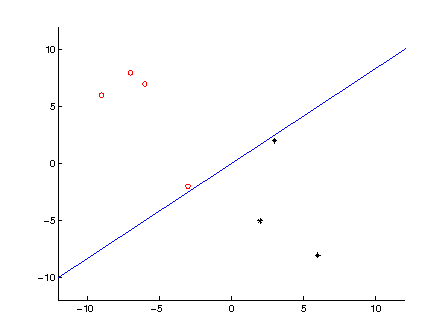
\includegraphics[width=1\textwidth]{plots/6_7}\caption{Problem 6 step 7}
\end{figure}
